\documentclass[a4paper]{article}

\usepackage[english]{babel}
\usepackage[utf8]{inputenc}
\usepackage{amsmath}
\usepackage{graphicx}
\usepackage{float}

\title{Photovaltaic effect}

\author{Jakob Huber 961130-3935\\ Viktor Nilsson 960217-}

\date{\today}

\begin{document}
\maketitle

\section{Introduction}

\[I=I_{sat}\left( 1 - exp\left( - \frac{eV}{nk_bT}\right) \right)\]\label{IV}

\section{Experimental procedure} 

    The cell used in the lab is a polycrystalline silicon thin film. Illumination is supplied by a standard desk lamp. A Power Cassy will measure the current. A modeling circuit as seen in figure, a simplification, illustrates the setting. The following relations are derived from the circuit $U=U_0-IR_0$ and $R=-U/I$ where the second is from the applied voltage acting as an external load. This leads to the power as $P=(-U)I$ done on the load. 

    The measurements consist firstly of one without applied bias, with illumination can be seen in the figure as without produces an uninteresting graph zero everywhere. Secondly getting the IV-characteristics, first with illumination where the IV curve is fitted \ref{IV} and without to identify "noise" and eliminate its effect by averaging. The last measurements are for determining the power vs distance relation, where the characteristics is measured with the lamp at different heights from the solar cell. I versus V and P versus V are plotted for all distances.
   
    Additionally a plot of the $P_{max}$, from the P vs V plots, versus $f(d)/f(0)$. Where $f$, the distance relation is derived from the spreading in a spherical manner from the light source thus being proportional to the inverse distance squared $f(d)=a/(d+b)^2$. Fitting parameters $a,b$ include a reference power at some known distance $a$ and a systematic distance offset $b$.  

\section{Results}

	 \begin{figure}
		\centering
		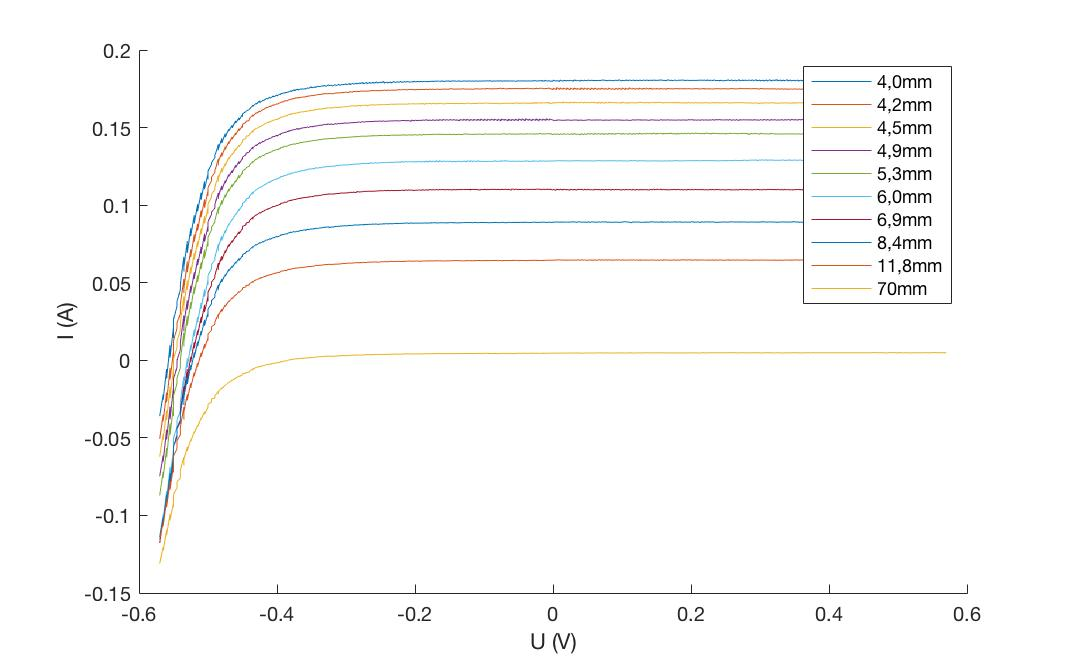
\includegraphics[width=1.1\textwidth]{dist_U-I}
		\caption{\label{fig:data1}}
	\end{figure}
	
	\begin{figure}
		\centering
		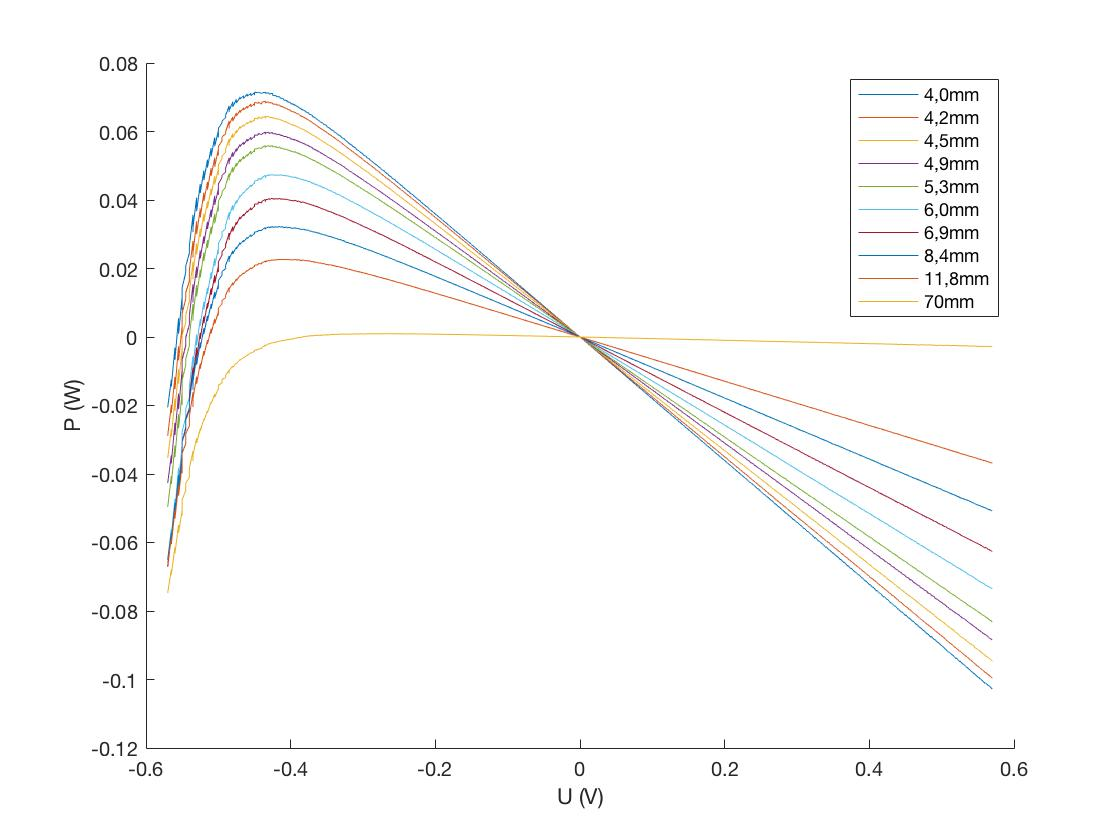
\includegraphics[width=1.1\textwidth]{dist_U-P}
		\caption{\label{fig:data2}}
	\end{figure}

\section{Discussion of the results}

	This is valid in the current setting as the fit is good.

\section{Conclusions}

Using the relations of the figure and given equations the formula becomes $P=\frac{U^2R}{(R+R_0)^2}$ for which the denominator has a minimum at $R=R_0$. Check derivatives


The photoelectric effect limits the frequency and a minimum is .
A sine-wave with a period of about 10(20?) ms is spotted. This is explained by the fact that the swedish power network is operating at 50 Hz and that the current generated by the solar cell is an increasing function of its absorbed power which is proportional to the power output of the lamp. 
The IV-characteristics of the solar cell fits the diode equation well as can be seen by looking at this graph. The fit admits an ideality factor of -49.5 mA. 

\begin{figure}
    \centering
%    \includegraphics[width=1\textwidth]{}
    \caption{\label{fig:data}}
\end{figure}

\end{document}